\documentclass[12pt]{article}
\usepackage[utf8]{inputenc}
\usepackage[left=2cm,right=2cm,top=2cm,bottom=2cm]{geometry}
\usepackage{graphicx, color, multicol, multirow}
\usepackage{float}
\usepackage[small]{caption}
\usepackage[spanish]{babel}
\usepackage{enumerate, amsmath, amssymb}
\usepackage{url}

%%%%%%%%%%%%%%%%%%%%%%%%%%%%%%%%%%%%%%%%%%%

\setlength{\parskip}{\baselineskip}
\spanishdecimal{.}

\begin{document}

%%%%%%%%%%%%%%%%%%%%%%%%%%%%%%%%%%%%%%%%%%
\thispagestyle{empty}
\hrule height2.5pt
\vspace{.1cm}
\hrule height1pt
%\vspace{.3cm}

\begin{center}
Tarea 1\\
Gabriela S\'anchez Y.\\
\end{center}

\vspace{.3cm}
\hrule height1pt
\vspace{.1cm}
\hrule height2.5pt
\vspace*{.5cm}
%%%%%%%%%%%%%%%%%%%%%%%%%%%%%%%%%%%%%%%%%%%%

En esta actividad se realiza un análisis descriptivo de la prevalencia delictiva en las entidades federativas del país en el periodo 2010-2018.

\section{Datos}

Los datos utilizados para el análisis se obtienen de la página del INEGI en la sección correspondiente a Seguridad pública y justicia \cite{inegi}. En este trabajo, únicamente se analiza la información acerca de la tasa de prevalencia delictiva por cada cien mil habitantes de cada una de las 32 entidades federativas del país, en el periodo comprendido entre los años 2010 a 2018.

%La información se muestra como una tasa por cada cien mil habitantes. %n los datos sobre victimización que el INEGI define como \textit{delito que afecta a una persona o a un hogar}. que afectó a los hogares mexicanos 

Los datos se guardan en un archivo \textsc{csv} y el análisis descriptivo se realiza con la ayuda del lenguaje de programación \textsc{R} versión 4.0.2 \cite{r}.


\section{Diagramas caja bigote}

En la figura \ref{vic} se observan los diagramas de caja bigote que resumen la información de la tasa de prevalencia delictiva por cada cien mil habitantes en cada una de las entidades federativas en el periodo 2010-2018. Es de esperarse que el Estado de México presente una mediana mayor al resto ya que es de los estados más poblado del país.

El INEGI también proporciona información de la tasa de prevalencia delictiva por cada cien mil habitantes según el sexo de la víctima, por lo que también es recopilada esa información para el Estado de Máxico. Se realiza este análisis porque anteriormente se observó que esta entidad presenta, en promedio, la mayor la tasa de incidencias delictivas. Esta última información se recopila directamente en un script de \textsc{R} (\textsc{t1.R}). La figura \ref{vic.edomex} muestra que, en promedio, la tasa de prevalencia delictiva en hombres es mayor en el caso de las mujeres. 


\begin{figure}
	\centering
	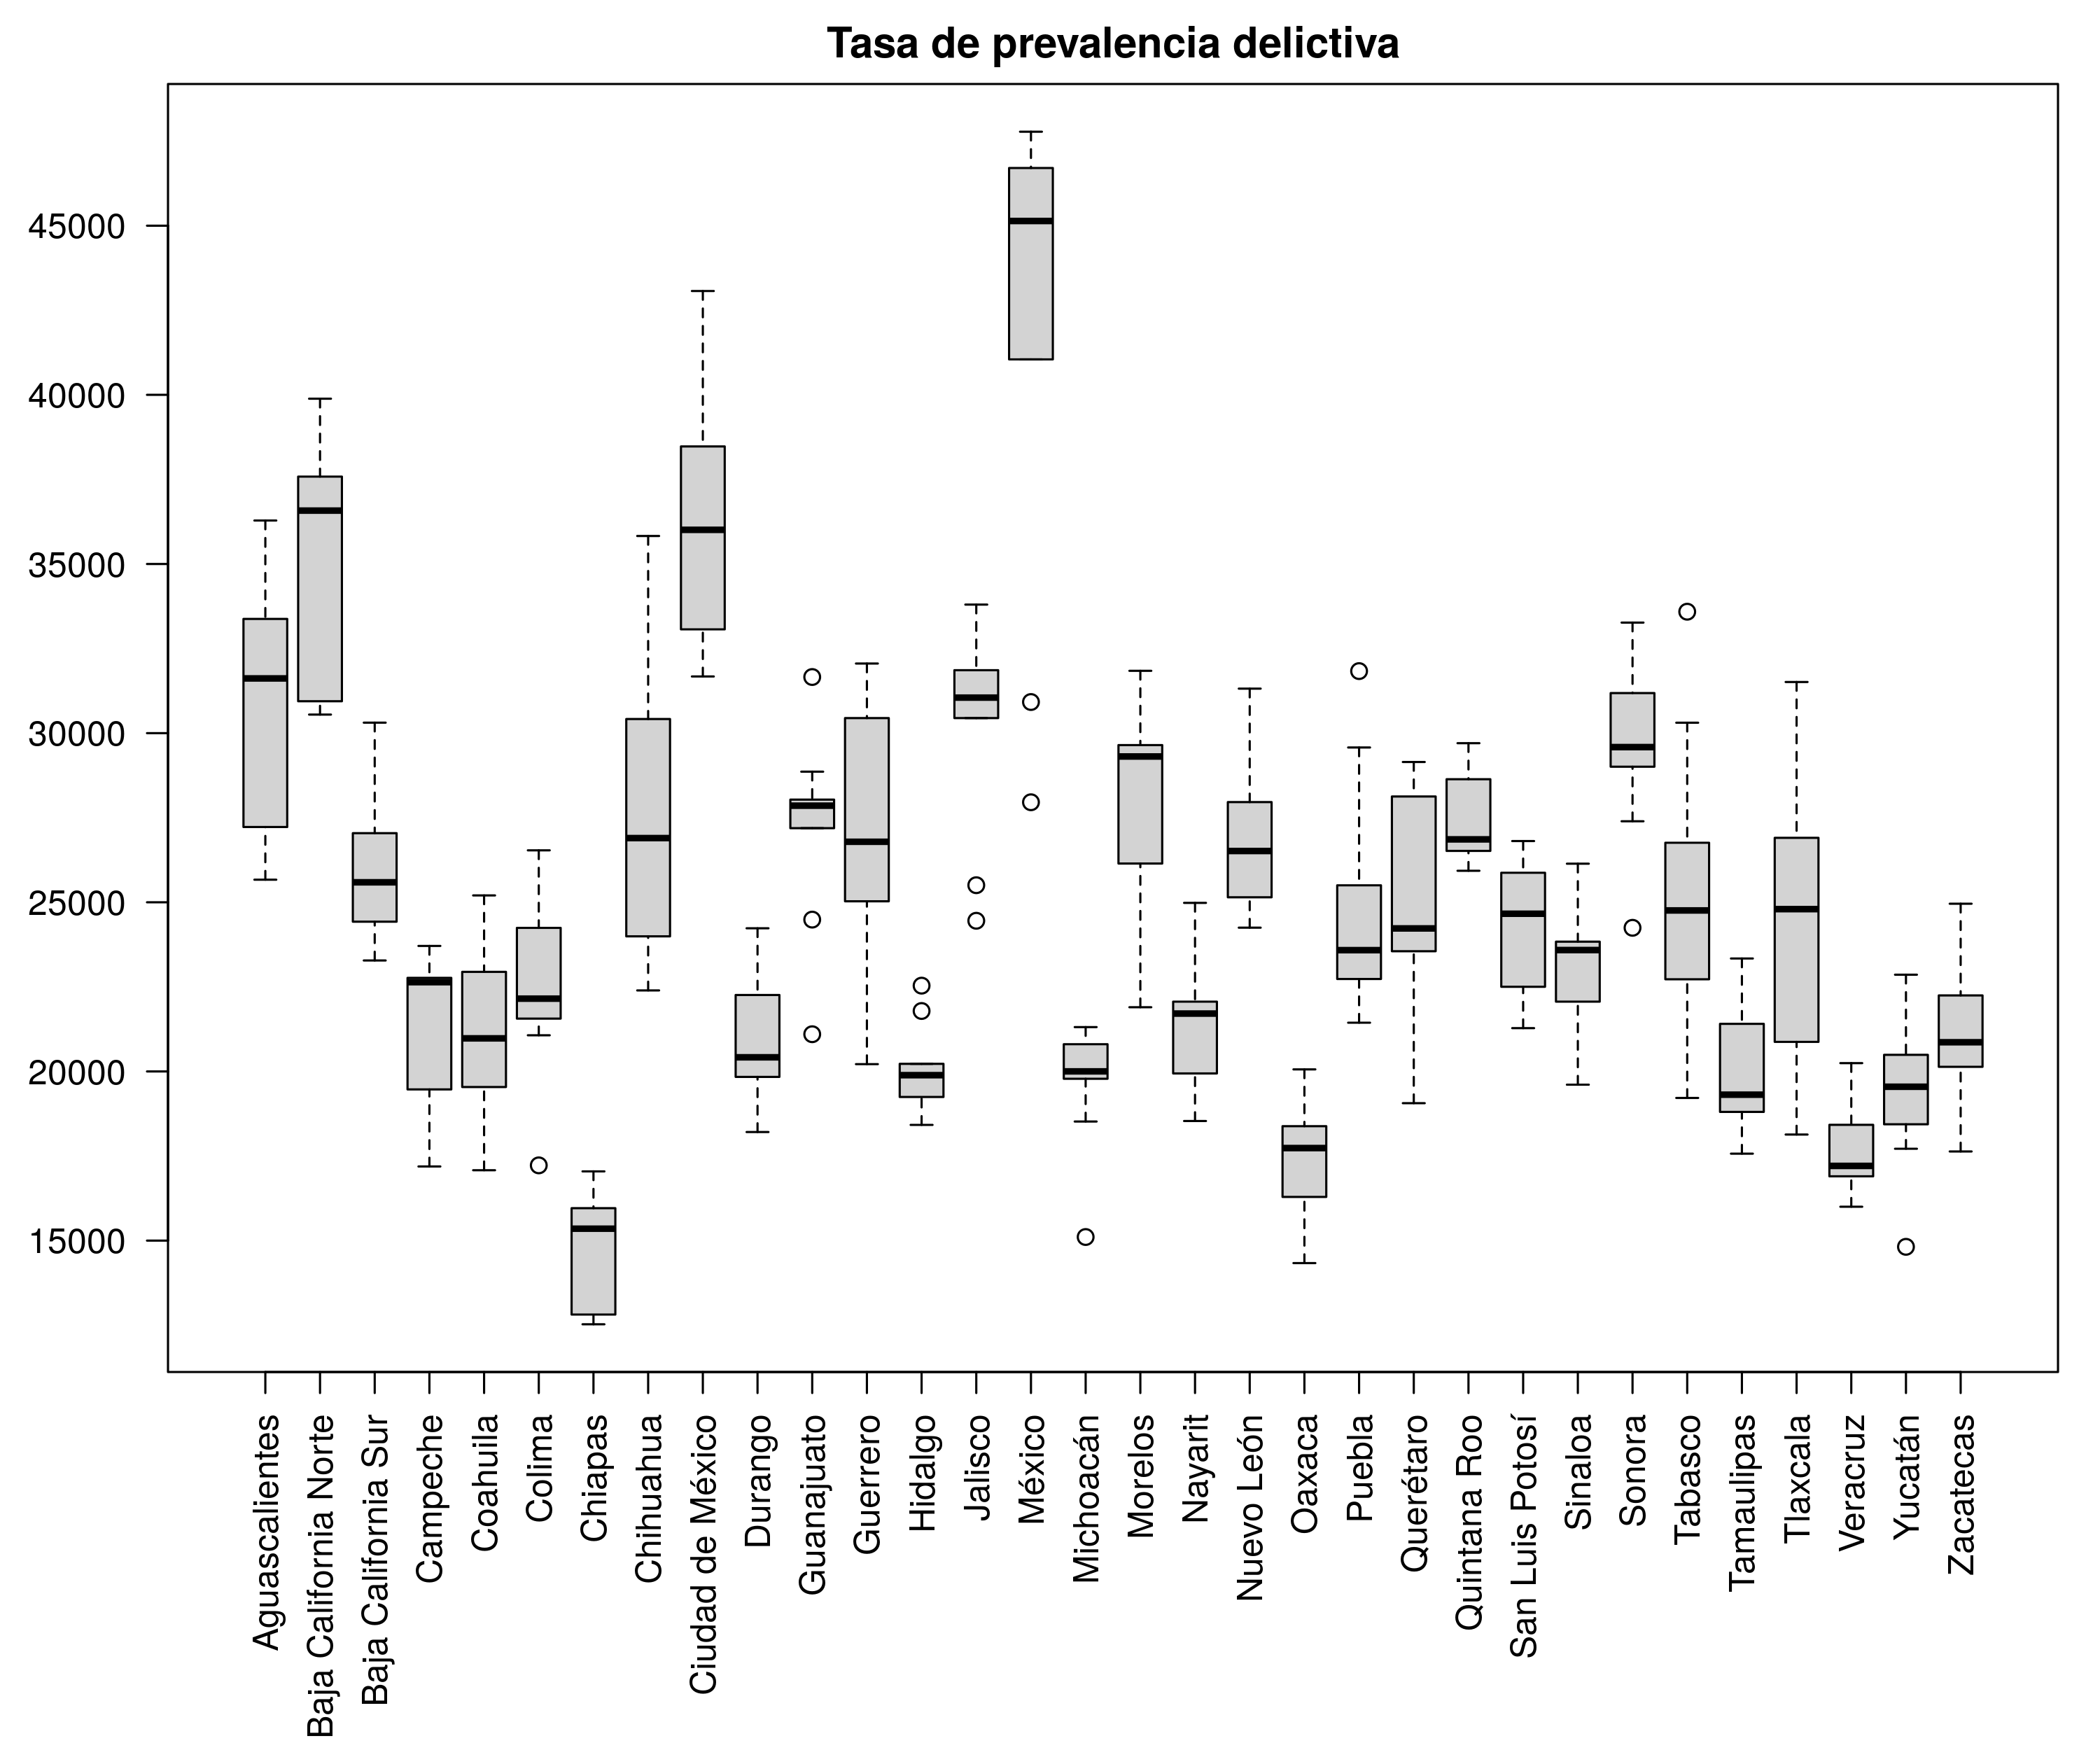
\includegraphics[scale=0.5]{victimizacion.png}
	\caption{Diagrama caja bigote de la tasa de prevalencia delictiva por cada cien mil habitantes en el periodo 2010-2018.}
	\label{vic}
\end{figure}

\begin{figure}
	\centering
	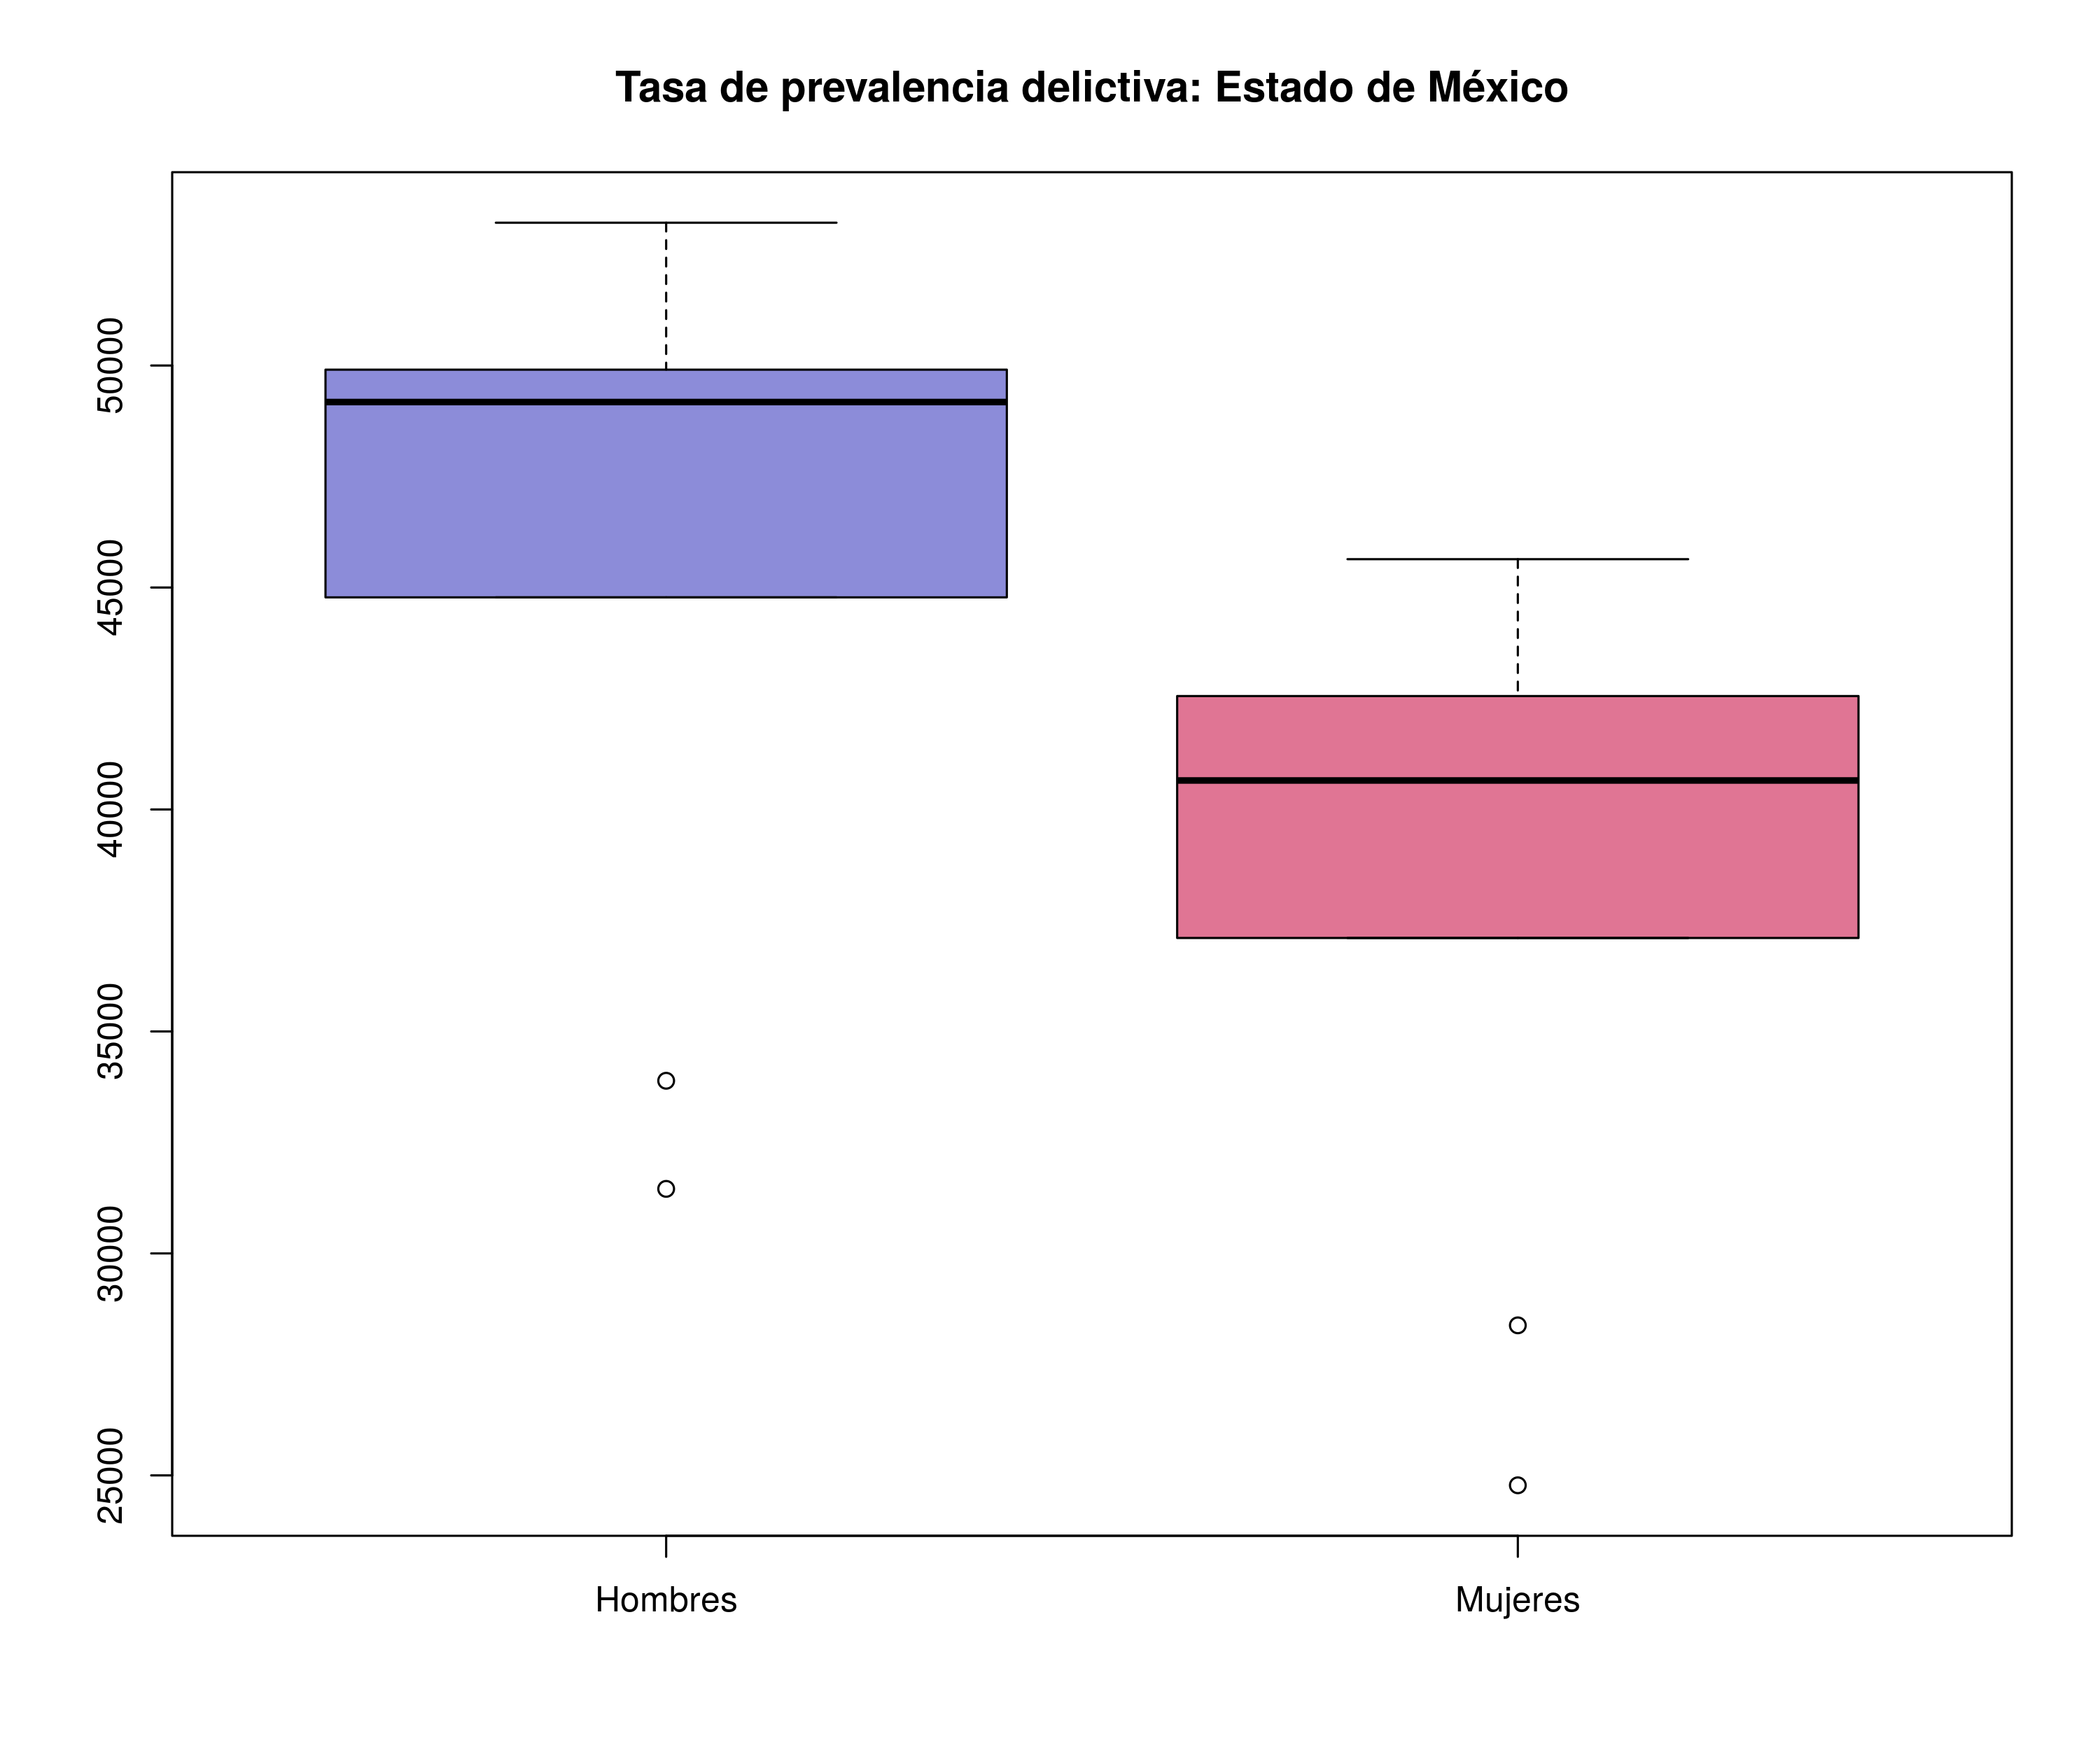
\includegraphics[scale=0.5]{edomex.png}
	\caption{Diagrama caja bigote de la tasa de prevalencia delictiva por cada cien mil habitantes, en el periodo 2010-2018, para el Estado de México según el sexo.}
	\label{vic.edomex}
\end{figure}

\nocite{*}
\bibliographystyle{plain}
\bibliography{biblio}



\end{document}

